\begin{figure}[H]
  \centering

  % color list kudos https://sashamaps.net/docs/resources/20-colors/
  \definecolor{color1}{HTML}{e6194b}
  \definecolor{color2}{HTML}{3cb44b}
  \definecolor{color3}{HTML}{ffe119}
  \definecolor{color4}{HTML}{4363d8}
  \definecolor{color5}{HTML}{f58231}
  \definecolor{color6}{HTML}{911eb4}
  \definecolor{color7}{HTML}{42d4f4}
  \definecolor{color8}{HTML}{f032e6}
  \definecolor{color9}{HTML}{bfef45}
  \definecolor{color10}{HTML}{fabed4}
  \definecolor{color11}{HTML}{469990}
  \definecolor{color12}{HTML}{dcbeff}
  \definecolor{color13}{HTML}{9a6324}
  \definecolor{color14}{HTML}{000075}
  \definecolor{color15}{HTML}{800000}
  \definecolor{color16}{HTML}{aaffc3}
  \definecolor{color17}{HTML}{808000}

  \tikzstyle{node}=[
	circle,
  draw,
  fill,
	minimum size=0.75cm,
  text=white,
	thick,
  ]

  \tikzstyle{style1}=[ draw=color1, fill=color1, text=white ]
  \tikzstyle{style2}=[ draw=color2, fill=color2, text=white ]
  \tikzstyle{style3}=[ draw=color3, fill=color3, text=black ]
  \tikzstyle{style4}=[ draw=color4, fill=color4, text=white ]
  \tikzstyle{style5}=[ draw=color5, fill=color5, text=white ]
  \tikzstyle{style6}=[ draw=color6, fill=color6, text=white ]
  \tikzstyle{style7}=[ draw=color7, fill=color7, text=black ]
  \tikzstyle{style8}=[ draw=color8, fill=color8, text=white ]
  \tikzstyle{style9}=[ draw=color9, fill=color9, text=black ]
  \tikzstyle{style10}=[ draw=color10, fill=color10, text=black ]
  \tikzstyle{style11}=[ draw=color11, fill=color11, text=white ]
  \tikzstyle{style12}=[ draw=color12, fill=color12, text=black ]
  \tikzstyle{style13}=[ draw=color13, fill=color13, text=white ]
  \tikzstyle{style14}=[ draw=color14, fill=color14, text=white ]
  \tikzstyle{style15}=[ draw=color15, fill=color15, text=white ]
  \tikzstyle{style16}=[ draw=color16, fill=color16, text=black ]
  \tikzstyle{style17}=[ draw=color17, fill=color17, text=white ]

  \tikzstyle{heavy edge}=[ very thick, ]

  \tikzstyle{light edge}=[ very thin, black!50, ]

  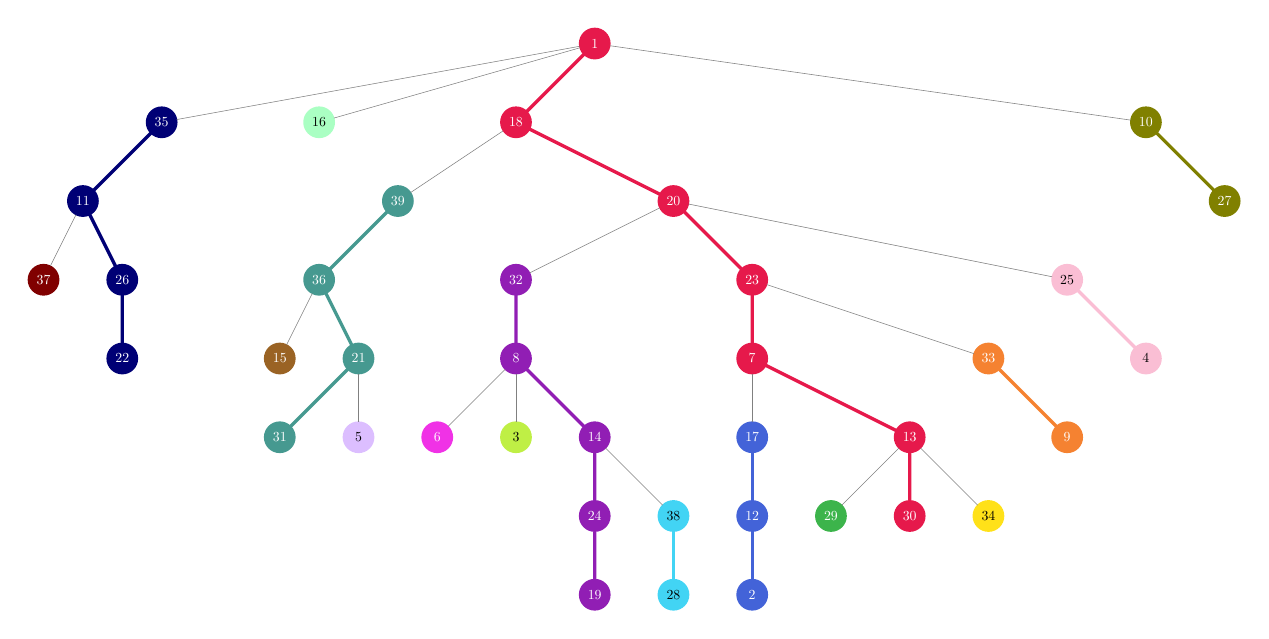
\begin{tikzpicture}[
    scale=0.5,
    every node/.style={scale=0.5},
    ]
    \node[node, style1] (n1) at (14,0) {$1$};
    \node[node, style14] (n35) at (3,-2) {$35$};
    \node[node, style14] (n11) at (1,-4) {$11$};
    \node[node, style15] (n37) at (0,-6) {$37$};
    \draw[light edge] (n11) -- (n37);

    \node[node, style14] (n26) at (2,-6) {$26$};
    \node[node, style14] (n22) at (2,-8) {$22$};
    \draw[light edge] (n1) -- (n35);
    \draw[heavy edge, style14] (n35) -- (n11) -- (n26) -- (n22);

    \node[node, style16] (n16) at (7,-2) {$16$};
    \draw[light edge] (n1) -- (n16);

    \node[node, style1] (n18) at (12,-2) {$18$};
    \node[node, style11] (n39) at (9,-4) {$39$};
    \node[node, style11] (n36) at (7,-6) {$36$};

    \node[node, style13] (n15) at (6,-8) {$15$};
    \draw[light edge] (n36) -- (n15);

    \node[node, style11] (n21) at (8,-8) {$21$};
    \node[node, style11] (n31) at (6,-10) {$31$};
    \draw[light edge] (n18) -- (n39);
    \draw[heavy edge, style11] (n39) -- (n36) -- (n21) -- (n31);

    \node[node, style12] (n5) at (8,-10) {$5$};
    \draw[light edge] (n21) -- (n5);

    \node[node, style1] (n20) at (16,-4) {$20$};
    \node[node, style6] (n32) at (12, -6) {$32$};
    \node[node, style6] (n8) at (12,-8) {$8$};
    \node[node, style8] (n6) at (10,-10) {$6$};
    \draw[light edge] (n8) -- (n6);

    \node[node, style9] (n3) at (12,-10) {$3$};
    \draw[light edge] (n8) -- (n3);

    \node[node, style6] (n14) at (14,-10) {$14$};
    \node[node, style6] (n24) at (14,-12) {$24$};
    \node[node, style6] (n19) at (14,-14) {$19$};
    \draw[light edge] (n20) -- (n32);
    \draw[heavy edge, style6] (n32) -- (n8) -- (n14) -- (n24) -- (n19);

    \node[node, style7] (n38) at (16,-12) {$38$};
    \node[node, style7] (n28) at (16,-14) {$28$};
    \draw[light edge] (n14) -- (n38);
    \draw[heavy edge, style7] (n38) -- (n28);

    \node[node, style1] (n23) at (18,-6) {$23$};
    \node[node, style1] (n7) at (18,-8) {$7$};

    \node[node, style4] (n17) at (18,-10) {$17$};
    \node[node, style4] (n12) at (18,-12) {$12$};
    \node[node, style4] (n2) at (18,-14) {$2$};
    \draw[light edge] (n7) -- (n17);
    \draw[heavy edge, style4] (n17) -- (n12) -- (n2);

    \node[node, style1] (n13) at (22,-10) {$13$};

    \node[node, style2] (n29) at (20,-12) {$29$};
    \draw[light edge] (n13) -- (n29);

    \node[node, style1] (n30) at (22,-12) {$30$};
    \draw[heavy edge, style1] (n1) -- (n18) -- (n20) -- (n23) -- (n7) -- (n13) -- (n30);

    \node[node, style3] (n34) at (24,-12) {$34$};
    \draw[light edge] (n13) -- (n34);

    \node[node, style5] (n33) at (24,-8) {$33$};
    \node[node, style5] (n9) at (26,-10) {$9$};
    \draw[light edge] (n23) -- (n33);
    \draw[heavy edge, style5] (n33) -- (n9);

    \node[node, style10] (n25) at (26,-6) {$25$};
    \node[node, style10] (n4) at (28,-8) {$4$};
    \draw[light edge] (n20) -- (n25);
    \draw[heavy edge, style10] (n25) -- (n4);

    \node[node, style17] (n10) at (28,-2) {$10$};
    \node[node, style17] (n27) at (30,-4) {$27$};
    \draw[light edge] (n1) -- (n10);
    \draw[heavy edge, style17] (n10) -- (n27);
  \end{tikzpicture}

  \caption{Un arbore în care muchia grea a fiecărui nod este îngroșată și colorată. Fiecare culoare indică un lanț de muchii grele consecutive.}
  \label{fig:tree-heavy-light-1}
\end{figure}
